% Created by tikzDevice version 0.12.3.1 on 2021-04-15 15:43:18
% !TEX encoding = UTF-8 Unicode
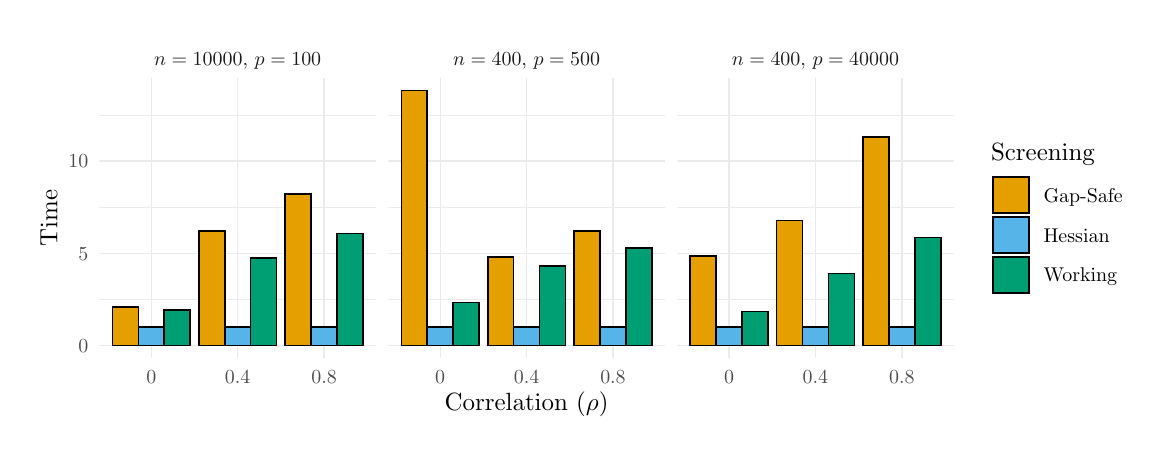
\begin{tikzpicture}[x=1pt,y=1pt]
\definecolor{fillColor}{RGB}{255,255,255}
\path[use as bounding box,fill=fillColor,fill opacity=0.00] (0,0) rectangle (404.71,144.54);
\begin{scope}
\path[clip] ( 25.95, 25.11) rectangle (125.84,126.48);
\definecolor{drawColor}{gray}{0.92}

\path[draw=drawColor,line width= 0.2pt,line join=round] ( 25.95, 46.38) --
	(125.84, 46.38);

\path[draw=drawColor,line width= 0.2pt,line join=round] ( 25.95, 79.71) --
	(125.84, 79.71);

\path[draw=drawColor,line width= 0.2pt,line join=round] ( 25.95,113.03) --
	(125.84,113.03);

\path[draw=drawColor,line width= 0.5pt,line join=round] ( 25.95, 29.71) --
	(125.84, 29.71);

\path[draw=drawColor,line width= 0.5pt,line join=round] ( 25.95, 63.04) --
	(125.84, 63.04);

\path[draw=drawColor,line width= 0.5pt,line join=round] ( 25.95, 96.37) --
	(125.84, 96.37);

\path[draw=drawColor,line width= 0.5pt,line join=round] ( 44.68, 25.11) --
	( 44.68,126.48);

\path[draw=drawColor,line width= 0.5pt,line join=round] ( 75.89, 25.11) --
	( 75.89,126.48);

\path[draw=drawColor,line width= 0.5pt,line join=round] (107.11, 25.11) --
	(107.11,126.48);
\definecolor{drawColor}{RGB}{0,0,0}
\definecolor{fillColor}{RGB}{230,159,0}

\path[draw=drawColor,line width= 0.6pt,line cap=rect,fill=fillColor] ( 30.63, 29.71) rectangle ( 39.99, 43.63);
\definecolor{fillColor}{RGB}{86,180,233}

\path[draw=drawColor,line width= 0.6pt,line cap=rect,fill=fillColor] ( 39.99, 29.71) rectangle ( 49.36, 36.38);
\definecolor{fillColor}{RGB}{0,158,115}

\path[draw=drawColor,line width= 0.6pt,line cap=rect,fill=fillColor] ( 49.36, 29.71) rectangle ( 58.72, 42.60);
\definecolor{fillColor}{RGB}{230,159,0}

\path[draw=drawColor,line width= 0.6pt,line cap=rect,fill=fillColor] ( 61.84, 29.71) rectangle ( 71.21, 71.00);
\definecolor{fillColor}{RGB}{86,180,233}

\path[draw=drawColor,line width= 0.6pt,line cap=rect,fill=fillColor] ( 71.21, 29.71) rectangle ( 80.57, 36.38);
\definecolor{fillColor}{RGB}{0,158,115}

\path[draw=drawColor,line width= 0.6pt,line cap=rect,fill=fillColor] ( 80.57, 29.71) rectangle ( 89.94, 61.41);
\definecolor{fillColor}{RGB}{230,159,0}

\path[draw=drawColor,line width= 0.6pt,line cap=rect,fill=fillColor] ( 93.06, 29.71) rectangle (102.42, 84.36);
\definecolor{fillColor}{RGB}{86,180,233}

\path[draw=drawColor,line width= 0.6pt,line cap=rect,fill=fillColor] (102.42, 29.71) rectangle (111.79, 36.38);
\definecolor{fillColor}{RGB}{0,158,115}

\path[draw=drawColor,line width= 0.6pt,line cap=rect,fill=fillColor] (111.79, 29.71) rectangle (121.15, 70.19);
\end{scope}
\begin{scope}
\path[clip] (130.34, 25.11) rectangle (230.23,126.48);
\definecolor{drawColor}{gray}{0.92}

\path[draw=drawColor,line width= 0.2pt,line join=round] (130.34, 46.38) --
	(230.23, 46.38);

\path[draw=drawColor,line width= 0.2pt,line join=round] (130.34, 79.71) --
	(230.23, 79.71);

\path[draw=drawColor,line width= 0.2pt,line join=round] (130.34,113.03) --
	(230.23,113.03);

\path[draw=drawColor,line width= 0.5pt,line join=round] (130.34, 29.71) --
	(230.23, 29.71);

\path[draw=drawColor,line width= 0.5pt,line join=round] (130.34, 63.04) --
	(230.23, 63.04);

\path[draw=drawColor,line width= 0.5pt,line join=round] (130.34, 96.37) --
	(230.23, 96.37);

\path[draw=drawColor,line width= 0.5pt,line join=round] (149.07, 25.11) --
	(149.07,126.48);

\path[draw=drawColor,line width= 0.5pt,line join=round] (180.28, 25.11) --
	(180.28,126.48);

\path[draw=drawColor,line width= 0.5pt,line join=round] (211.50, 25.11) --
	(211.50,126.48);
\definecolor{drawColor}{RGB}{0,0,0}
\definecolor{fillColor}{RGB}{230,159,0}

\path[draw=drawColor,line width= 0.6pt,line cap=rect,fill=fillColor] (135.02, 29.71) rectangle (144.38,121.87);
\definecolor{fillColor}{RGB}{86,180,233}

\path[draw=drawColor,line width= 0.6pt,line cap=rect,fill=fillColor] (144.38, 29.71) rectangle (153.75, 36.38);
\definecolor{fillColor}{RGB}{0,158,115}

\path[draw=drawColor,line width= 0.6pt,line cap=rect,fill=fillColor] (153.75, 29.71) rectangle (163.11, 45.17);
\definecolor{fillColor}{RGB}{230,159,0}

\path[draw=drawColor,line width= 0.6pt,line cap=rect,fill=fillColor] (166.23, 29.71) rectangle (175.60, 61.70);
\definecolor{fillColor}{RGB}{86,180,233}

\path[draw=drawColor,line width= 0.6pt,line cap=rect,fill=fillColor] (175.60, 29.71) rectangle (184.96, 36.38);
\definecolor{fillColor}{RGB}{0,158,115}

\path[draw=drawColor,line width= 0.6pt,line cap=rect,fill=fillColor] (184.96, 29.71) rectangle (194.33, 58.42);
\definecolor{fillColor}{RGB}{230,159,0}

\path[draw=drawColor,line width= 0.6pt,line cap=rect,fill=fillColor] (197.45, 29.71) rectangle (206.81, 71.03);
\definecolor{fillColor}{RGB}{86,180,233}

\path[draw=drawColor,line width= 0.6pt,line cap=rect,fill=fillColor] (206.81, 29.71) rectangle (216.18, 36.38);
\definecolor{fillColor}{RGB}{0,158,115}

\path[draw=drawColor,line width= 0.6pt,line cap=rect,fill=fillColor] (216.18, 29.71) rectangle (225.54, 64.96);
\end{scope}
\begin{scope}
\path[clip] (234.73, 25.11) rectangle (334.61,126.48);
\definecolor{drawColor}{gray}{0.92}

\path[draw=drawColor,line width= 0.2pt,line join=round] (234.73, 46.38) --
	(334.61, 46.38);

\path[draw=drawColor,line width= 0.2pt,line join=round] (234.73, 79.71) --
	(334.61, 79.71);

\path[draw=drawColor,line width= 0.2pt,line join=round] (234.73,113.03) --
	(334.61,113.03);

\path[draw=drawColor,line width= 0.5pt,line join=round] (234.73, 29.71) --
	(334.61, 29.71);

\path[draw=drawColor,line width= 0.5pt,line join=round] (234.73, 63.04) --
	(334.61, 63.04);

\path[draw=drawColor,line width= 0.5pt,line join=round] (234.73, 96.37) --
	(334.61, 96.37);

\path[draw=drawColor,line width= 0.5pt,line join=round] (253.45, 25.11) --
	(253.45,126.48);

\path[draw=drawColor,line width= 0.5pt,line join=round] (284.67, 25.11) --
	(284.67,126.48);

\path[draw=drawColor,line width= 0.5pt,line join=round] (315.89, 25.11) --
	(315.89,126.48);
\definecolor{drawColor}{RGB}{0,0,0}
\definecolor{fillColor}{RGB}{230,159,0}

\path[draw=drawColor,line width= 0.6pt,line cap=rect,fill=fillColor] (239.41, 29.71) rectangle (248.77, 61.92);
\definecolor{fillColor}{RGB}{86,180,233}

\path[draw=drawColor,line width= 0.6pt,line cap=rect,fill=fillColor] (248.77, 29.71) rectangle (258.14, 36.38);
\definecolor{fillColor}{RGB}{0,158,115}

\path[draw=drawColor,line width= 0.6pt,line cap=rect,fill=fillColor] (258.14, 29.71) rectangle (267.50, 41.97);
\definecolor{fillColor}{RGB}{230,159,0}

\path[draw=drawColor,line width= 0.6pt,line cap=rect,fill=fillColor] (270.62, 29.71) rectangle (279.99, 74.92);
\definecolor{fillColor}{RGB}{86,180,233}

\path[draw=drawColor,line width= 0.6pt,line cap=rect,fill=fillColor] (279.99, 29.71) rectangle (289.35, 36.38);
\definecolor{fillColor}{RGB}{0,158,115}

\path[draw=drawColor,line width= 0.6pt,line cap=rect,fill=fillColor] (289.35, 29.71) rectangle (298.72, 55.74);
\definecolor{fillColor}{RGB}{230,159,0}

\path[draw=drawColor,line width= 0.6pt,line cap=rect,fill=fillColor] (301.84, 29.71) rectangle (311.20,105.01);
\definecolor{fillColor}{RGB}{86,180,233}

\path[draw=drawColor,line width= 0.6pt,line cap=rect,fill=fillColor] (311.20, 29.71) rectangle (320.57, 36.38);
\definecolor{fillColor}{RGB}{0,158,115}

\path[draw=drawColor,line width= 0.6pt,line cap=rect,fill=fillColor] (320.57, 29.71) rectangle (329.93, 68.74);
\end{scope}
\begin{scope}
\path[clip] ( 25.95,126.48) rectangle (125.84,140.04);
\definecolor{drawColor}{gray}{0.10}

\node[text=drawColor,anchor=base,inner sep=0pt, outer sep=0pt, scale=  0.72] at ( 75.89,130.78) {$n=10000$, $p=100$};
\end{scope}
\begin{scope}
\path[clip] (130.34,126.48) rectangle (230.23,140.04);
\definecolor{drawColor}{gray}{0.10}

\node[text=drawColor,anchor=base,inner sep=0pt, outer sep=0pt, scale=  0.72] at (180.28,130.78) {$n=400$, $p=500$};
\end{scope}
\begin{scope}
\path[clip] (234.73,126.48) rectangle (334.61,140.04);
\definecolor{drawColor}{gray}{0.10}

\node[text=drawColor,anchor=base,inner sep=0pt, outer sep=0pt, scale=  0.72] at (284.67,130.78) {$n=400$, $p=40000$};
\end{scope}
\begin{scope}
\path[clip] (  0.00,  0.00) rectangle (404.71,144.54);
\definecolor{drawColor}{gray}{0.30}

\node[text=drawColor,anchor=base,inner sep=0pt, outer sep=0pt, scale=  0.72] at ( 44.68, 16.10) {0};

\node[text=drawColor,anchor=base,inner sep=0pt, outer sep=0pt, scale=  0.72] at ( 75.89, 16.10) {0.4};

\node[text=drawColor,anchor=base,inner sep=0pt, outer sep=0pt, scale=  0.72] at (107.11, 16.10) {0.8};
\end{scope}
\begin{scope}
\path[clip] (  0.00,  0.00) rectangle (404.71,144.54);
\definecolor{drawColor}{gray}{0.30}

\node[text=drawColor,anchor=base,inner sep=0pt, outer sep=0pt, scale=  0.72] at (149.07, 16.10) {0};

\node[text=drawColor,anchor=base,inner sep=0pt, outer sep=0pt, scale=  0.72] at (180.28, 16.10) {0.4};

\node[text=drawColor,anchor=base,inner sep=0pt, outer sep=0pt, scale=  0.72] at (211.50, 16.10) {0.8};
\end{scope}
\begin{scope}
\path[clip] (  0.00,  0.00) rectangle (404.71,144.54);
\definecolor{drawColor}{gray}{0.30}

\node[text=drawColor,anchor=base,inner sep=0pt, outer sep=0pt, scale=  0.72] at (253.45, 16.10) {0};

\node[text=drawColor,anchor=base,inner sep=0pt, outer sep=0pt, scale=  0.72] at (284.67, 16.10) {0.4};

\node[text=drawColor,anchor=base,inner sep=0pt, outer sep=0pt, scale=  0.72] at (315.89, 16.10) {0.8};
\end{scope}
\begin{scope}
\path[clip] (  0.00,  0.00) rectangle (404.71,144.54);
\definecolor{drawColor}{gray}{0.30}

\node[text=drawColor,anchor=base east,inner sep=0pt, outer sep=0pt, scale=  0.72] at ( 21.90, 27.24) {0};

\node[text=drawColor,anchor=base east,inner sep=0pt, outer sep=0pt, scale=  0.72] at ( 21.90, 60.56) {5};

\node[text=drawColor,anchor=base east,inner sep=0pt, outer sep=0pt, scale=  0.72] at ( 21.90, 93.89) {10};
\end{scope}
\begin{scope}
\path[clip] (  0.00,  0.00) rectangle (404.71,144.54);
\definecolor{drawColor}{RGB}{0,0,0}

\node[text=drawColor,anchor=base,inner sep=0pt, outer sep=0pt, scale=  0.90] at (180.28,  6.25) {Correlation ($\rho$)};
\end{scope}
\begin{scope}
\path[clip] (  0.00,  0.00) rectangle (404.71,144.54);
\definecolor{drawColor}{RGB}{0,0,0}

\node[text=drawColor,rotate= 90.00,anchor=base,inner sep=0pt, outer sep=0pt, scale=  0.90] at ( 10.70, 75.79) {Time};
\end{scope}
\begin{scope}
\path[clip] (  0.00,  0.00) rectangle (404.71,144.54);
\definecolor{drawColor}{RGB}{0,0,0}

\node[text=drawColor,anchor=base west,inner sep=0pt, outer sep=0pt, scale=  0.90] at (348.11, 96.63) {Screening};
\end{scope}
\begin{scope}
\path[clip] (  0.00,  0.00) rectangle (404.71,144.54);
\definecolor{drawColor}{RGB}{0,0,0}
\definecolor{fillColor}{RGB}{230,159,0}

\path[draw=drawColor,line width= 0.6pt,line cap=rect,fill=fillColor] (348.83, 77.51) rectangle (361.86, 90.54);
\end{scope}
\begin{scope}
\path[clip] (  0.00,  0.00) rectangle (404.71,144.54);
\definecolor{drawColor}{RGB}{0,0,0}
\definecolor{fillColor}{RGB}{86,180,233}

\path[draw=drawColor,line width= 0.6pt,line cap=rect,fill=fillColor] (348.83, 63.05) rectangle (361.86, 76.09);
\end{scope}
\begin{scope}
\path[clip] (  0.00,  0.00) rectangle (404.71,144.54);
\definecolor{drawColor}{RGB}{0,0,0}
\definecolor{fillColor}{RGB}{0,158,115}

\path[draw=drawColor,line width= 0.6pt,line cap=rect,fill=fillColor] (348.83, 48.60) rectangle (361.86, 61.63);
\end{scope}
\begin{scope}
\path[clip] (  0.00,  0.00) rectangle (404.71,144.54);
\definecolor{drawColor}{RGB}{0,0,0}

\node[text=drawColor,anchor=base west,inner sep=0pt, outer sep=0pt, scale=  0.72] at (367.07, 81.54) {Gap-Safe};
\end{scope}
\begin{scope}
\path[clip] (  0.00,  0.00) rectangle (404.71,144.54);
\definecolor{drawColor}{RGB}{0,0,0}

\node[text=drawColor,anchor=base west,inner sep=0pt, outer sep=0pt, scale=  0.72] at (367.07, 67.09) {Hessian};
\end{scope}
\begin{scope}
\path[clip] (  0.00,  0.00) rectangle (404.71,144.54);
\definecolor{drawColor}{RGB}{0,0,0}

\node[text=drawColor,anchor=base west,inner sep=0pt, outer sep=0pt, scale=  0.72] at (367.07, 52.64) {Working};
\end{scope}
\end{tikzpicture}
